\documentclass[journal]{IEEEtran}

\usepackage{cite}
\usepackage{amsmath}
\interdisplaylinepenalty=2500
\usepackage{algorithm}
\usepackage[noend]{algpseudocode}
\usepackage{array}
\usepackage{graphicx}
\usepackage{float}

% correct bad hyphenation here
\hyphenation{op-tical net-works semi-conduc-tor}


\begin{document}
\title{Camera calibration with iterative refining of control points}

\author{Wilbert~Pumacay,~\textit{Catholic University San Pablo},~wilbert.pumacay@ucsp.edu.pe\\
        Gerson~Vizcarra,~\textit{Catholic University San Pablo},~gerson.vizcarra@ucsp.edu.pe}

% make the title area
\maketitle

\begin{abstract}
This paper presents an application of Prakash camera calibration approach \cite{Prakash2012}, that is a improvement of Ankur's one \cite{Ankur2009}, to get better results than Zhang \cite{CameraCalibration1} camera calibration technique implemented by OpenCV. Also we present an algorithm to detect rings pattern using adaptive segmentation, ellipse fitting, blob detector and other techniques. We present a comparison between results using feature extraction of chessboard corners, asymmetric circle grids, and concentric circle grid patterns, the first two, using functions implemented in OpenCV and the third one using our own algorithm.
\\
\\
In the presented method, we use an iterative approach, that relies on refinement of control points in grid patterns. First, we make an initial calibration using OpenCV implementation of Zhang's method, the captured images of patterns are undistorted and projected onto a fronto-parallel plane, then we detect points of control projecting and re-distorting them onto the original image to refine previous points of control. This process is repeated until a convergence between projected points and previous ones. The results show that the presented method reduces error in ... compared to OpenCV.

\end{abstract}

\begin{IEEEkeywords}
Camera calibration, calibration pattern, circle grid, image processing.
\end{IEEEkeywords}


\section{Introduction}

\IEEEPARstart{T}{he} camera calibration process is an important step in several applications, like augmented reality. To do calibration properly using current calibration methods we need to get features we can related in both 2D camera space and 3D world space to estimate the camera parameters that give this mapping. In this context, the use of grid patterns help by giving us the features we need, being the components in the pattern which we must detect in every frame in video.
\\
\\
The camera calibration problem consists of finding 11 parameters that describe the mapping between 2D camera space and 3D world space. Six parameters, called extrinsic, come from an homogeneous transform, giving 6 parameters ( rotation and translation around the axes ). The other 5 parameters, called intrinsic, define some internal properties of the camera. This can be expressed in the following transformation equation:

\begin{equation}
  \begin{bmatrix}
    \mu \\
    \nu \\
      1
  \end{bmatrix} =
  \begin{bmatrix}
    \alpha & \gamma & \mu_{0} \\
       0   & \beta  & \nu_{0} \\
       0   &    0   &    1
  \end{bmatrix}
  \begin{bmatrix}
    r_{x_{1}} & r_{y_{1}} & r_{z_{1}} & t_{x}\\
    r_{x_{2}} & r_{y_{2}} & r_{z_{2}} & t_{y}\\
    r_{x_{3}} & r_{y_{3}} & r_{z_{3}} & t_{z}
  \end{bmatrix}
  \begin{bmatrix}
    x \\
    y \\
    z \\
    1
  \end{bmatrix}
%
\end{equation}

In this equation we can detail each of the variables: $x,y,z$ are original coordinates of an object, $r_{ij}$ and $t_{ij}$ means the rotation and translation values respectively in the model matrix, $\alpha$ and $\beta$ represents the focal length in x and y axis respectively, $\mu_0$ and $\nu_0$ are the coordinates x and y at the optical center.
\\
\\
To find these parameters, camera calibration methods make use of correspondences between 2D and 3D spaces in order to fit the parameters that best describe this mapping. We achieve this by minimizing the following function:

\begin{equation}
  \sum^{m}_{i} \sum^{n}_{j} \Vert TP^{ij}_{3D} - P^{ij}_{2D} \Vert^{2}
\end{equation}

Where we are trying to minimize the difference between the expected projection and the actual projection over some set of features. The key idea is that supplying sufficient features that have a correct mapping, we can get the 11 parameters needed that minimize this function. So, a key part is the detection of these features.
\\
\\
In equation $2$ we are looping through a set of features $n$ that are found in each frame of a video of $m$ frames, so, we basically need to detect some feature points in each frame of video, which is what we focus in this paper.
\\
\\
This paper presents a camera calibration method that consist on iterative refinement of the camera calibration parameters by projection and unprojection to a fronto-parallel plane, and the localization of points of control combining adaptive thresholding and ellipse fitting to get better results.

\section{Related work}


\section{About the method}
The presented method starts from a initial Zhang's camera calibration process using three patterns: Chessboard, Asymmetric circles, and Rings; the first two using implemented functions of OpenCV and the third one, using our own implementation. The structure of our applied pipeline are described in Fig. 1.

\begin{figure}[H]
\centering
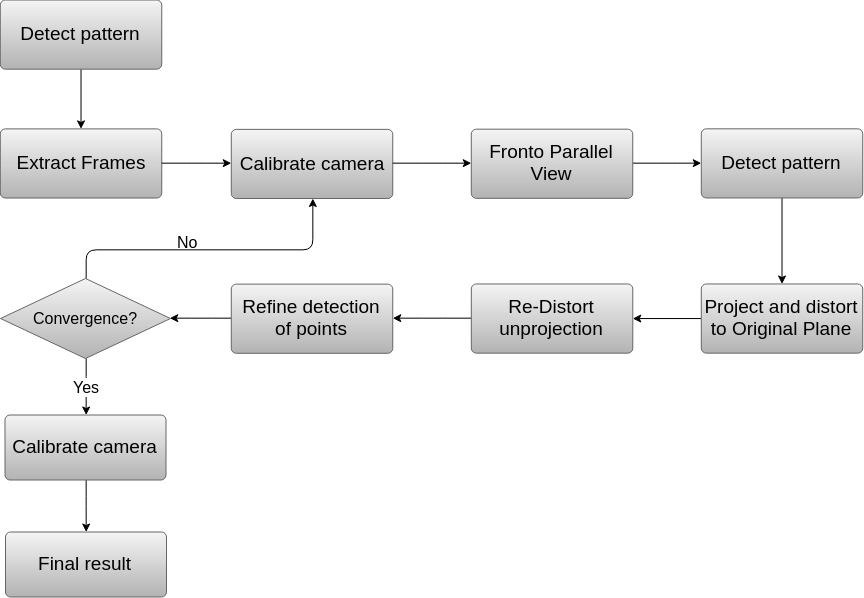
\includegraphics[width=3.0in]{_img/img_report4_pipeline.png}
\caption{Pipeline of the implementation.}
\end{figure}

\subsection{Circle concentric pattern detection}
In order to detect the pattern faster and get better results, we created a mode based detector, with three main modes: Finding Mode which has the function of detect the pattern in first frames, Tracking mode to track the order of recognized points and speed up the execution, and Recovering mode that is an temporal mode if there where a lost point in new Frame. In Fig. 2 we describe the modes in a chart.
\\
\\
Also, for detecting the points in pattern we used the pipeline specified in Fig. 2.
\begin{figure}[H]
\centering
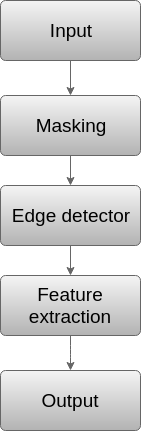
\includegraphics[width=0.7in]{_img/img_report4_pipeline_detector.png}
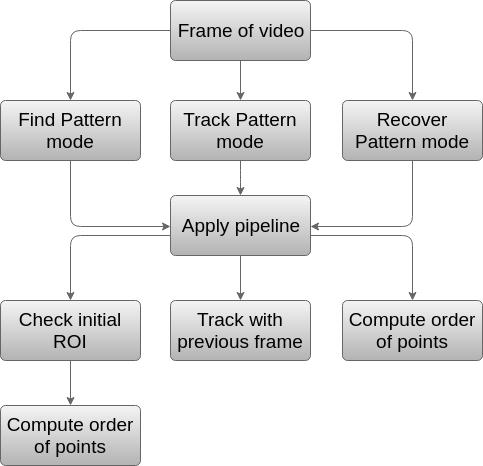
\includegraphics[width=2.3in]{_img/img_report4_pipeline_modes.png}
\caption{Left: pipeline of pattern detection. Right: Behavior of mode based detector.}
\end{figure}



\subsubsection{ Masking }
This step is in charge of isolating the pattern by using thresholding operations.
\\
\\
The approach consists on creating a mask from the grayscale transformed image applying \textbf{Adaptive Thresholding algorithm}, this algorithm relies on Integral Image technique specified in \cite{IntegralImageThresholding}.
\begin{algorithm}
\caption{Masking}
\label{alg:mask2}
\begin{algorithmic}[1]
\State $\textit{Set up thresholding parameters}$
\State $mask   = \textit{rgb2gray}( inputImage )$
\State $mask   = \textit{AdaptiveThreshold}(mask, blockSize)$\\
\Return $masked$
\end{algorithmic}
\end{algorithm}
%%%%%%%%%%%%%%%%%%%%%%%%%%%%%%%%%%%%%%%%%%%%%%%%%%%%%%%
\begin{figure}[H]
\centering
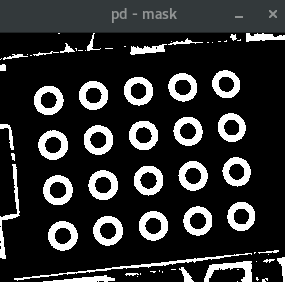
\includegraphics[width=2.5in]{_img/img_report2_mask.png}
\caption{Image mask applied to ROI.}
\end{figure}

\subsubsection{Edge detection}
In this stage of the pipeline we extract edges from the result of the previous stage. In order to do this, we applied \textbf{Scharr operators} on \textit{x} and \textit{y} axis (as described in algorithm 2); Scharr is the result from Sobel algorithm minimizing weighted mean squared angular error in Fourier domain.
%% TODO: Gerson
\begin{algorithm}
\caption{Edge detection}
\begin{algorithmic}[1]
\State $axis_x   = \textit{Scharr}(masked, 1, 0)$
\State $axis_x   = \textit{Abs}(axis_x)$
\State $axis_y   = \textit{Scharr}(masked, 0, 1)$
\State $axis_y   = \textit{Abs}(axis_y)$
\State $edgesImage   = \textit{Add}(axis_x, axis_y)$ \\
\Return $edgesImage$
\end{algorithmic}
\end{algorithm}

\begin{figure}[H]
\centering
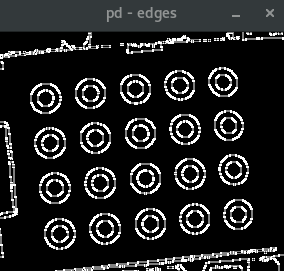
\includegraphics[width=2.5in]{_img/img_report2_edges.png}
\caption{Edge detection to mask.}
\end{figure}

\subsubsection{Feature extraction}
The last stage consist of extracting the features needed for the calibration from the edges detected in the previous stage. We used OpenCV's \textbf{SimpleBlobDetector} that applies an extra thresholding on the image, applies the \textbf{findContours} algorithm to calculate the blob centers, groups centers of several images by their coordinates in blobs and finally, estimates the final centers of the blobs. For detecting only pattern blobs, we had to apply similar heuristics to above (color blobs, area, aspect ratio, and convexity of points).

\begin{figure}[H]
\centering
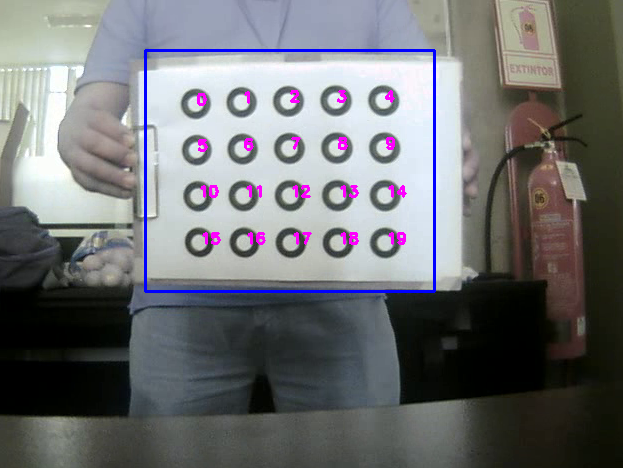
\includegraphics[width=2.5in]{_img/img_report2_feature_detection.png}
\caption{Result after feature detection.}
\end{figure}

\subsection{Pattern Matching and Ordering}
Once we have the features extracted, we have to order them for them to be used in the calibration algorithm. To achieve this, we made a simple algorithm that matches the best candidate grid to the current features, and correct by the orientation in order to choose a correct ordering.
\\
\\
We first create a bounding box of the current possible corners. Then, we take the outer most corners as the corners of the pattern. With this information, we can compute a candidate grid that represents the positions where the candidate points should be, as seen in figure 7.

\begin{figure}[H]
\centering
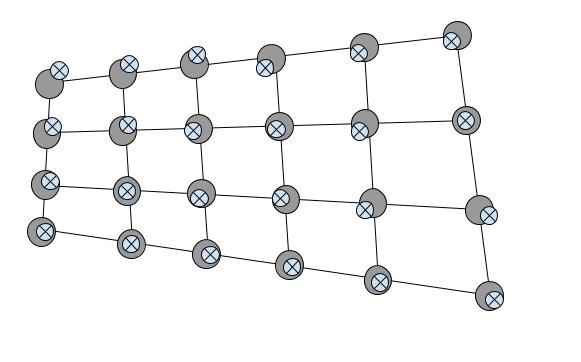
\includegraphics[width=2.5in]{_img/img_report3_pattern_matching.jpg}
\caption{Grid pattern matching.}
\end{figure}

We check for each combination of outer most corners, which ordering gives the best fit. This will give us a correct ordering of the outer most corners of the pattern.
\\
\\
Lastly, we check that the orientation of the board is in some range, as shown in figure 8, which will complete the corner ordering, as shown in figure 9.
\\
\\
\begin{figure}[H]
\centering
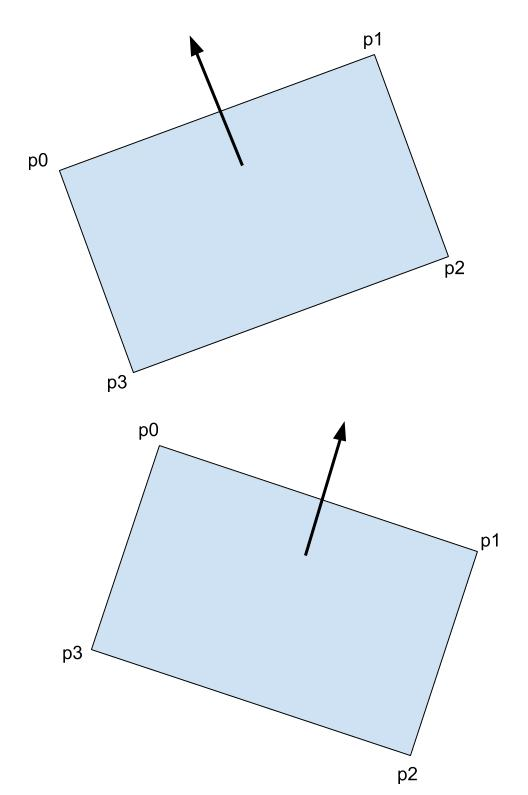
\includegraphics[width=2.5in]{_img/img_pattern_orientation_checking.jpg}
\caption{Pattern orientation check.}
\end{figure}

\begin{figure}[H]
\centering
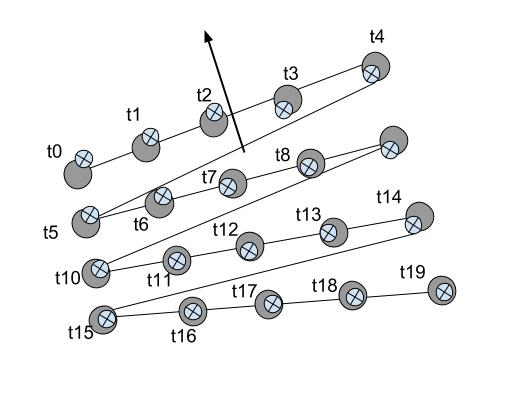
\includegraphics[width=2.5in]{_img/img_report3_pattern_order_check.jpg}
\caption{Pattern final ordering after matching.}
\end{figure}

\subsection{Calibration process}
To do camera calibration process, we took some frames using tools to show the distribution of points in frames in order to improve results: better calibration requires better distribution of points.
\\
\\
We used 30 calibration frames trying to distribute points location as max as possible. In figure 9 we show screenshots of heatmap and point distribution of a calibration process.

\begin{figure}[H]
\centering
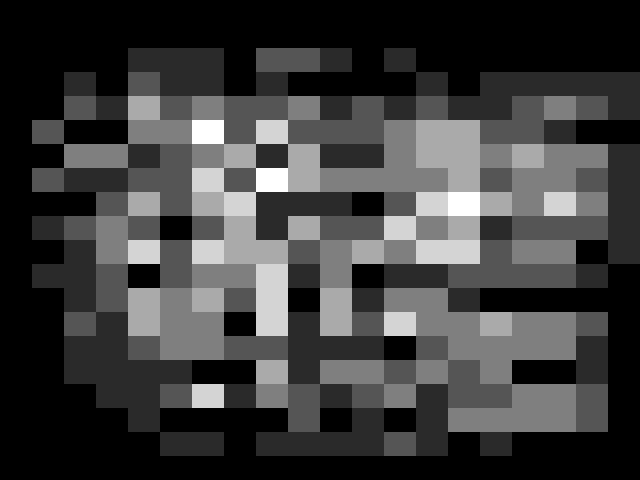
\includegraphics[width=1.5in]{_img/img_report3_heatmap.png}
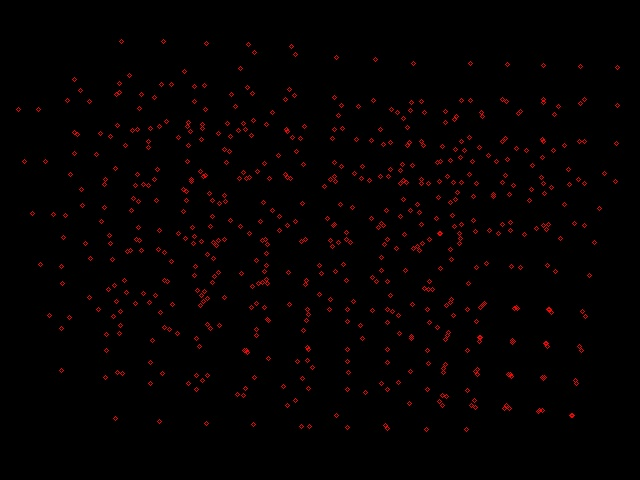
\includegraphics[width=1.5in]{_img/img_report3_points_distribution.png}
\caption{Left: Heatmap. Right: Points distribution.}
\end{figure}

Also we created a screen that shows the angle histogram of taken frames, like previous tools, it helps us to distribute angles better.
\begin{figure}[H]
\centering
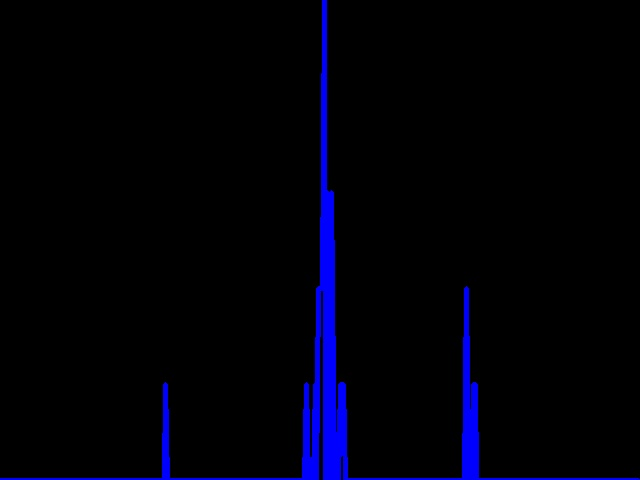
\includegraphics[width=1.5in]{_img/img_report3_angle_histogram.png}
\caption{Angle distribution histogram screen.}
\end{figure}

\section{Results}
We calibrated two cameras using as feature detection the three detection algorithms described earlier ( OpenCV's chessboard and circle finder and our algorithm )

For each calibration, we took a fixed batch of 30 correctly processed images. The results are the following:
\\
\\
\begin{table}[h]
\centering
\begin{tabular}{ |c||c|c|c|c|c|c|c|  }
 \hline
 Parameter & \multicolumn{3}{c|}{PS3 Eye cam} & \multicolumn{3}{c|}{MS lifecam}\\
 \cline{2-7}
 & Chessboard & Circles & Rings & Chessboard & Circles & Rings \\
 \hline
 fx        & 876.2 & 933.2 & 829.5 & 609.6 & 609.5 & 627.0\\
 fy        & 876.6 & 935.4 & 834.8 & 609.4 & 612.6 & 631.8\\
 vx        & 325.0 & 342.3 & 320.0 & 326.9 & 351.5 & 342.7\\
 vy 	       & 251.4 & 220.7 & 243.5 & 223.8 & 227.2 & 231.2\\
 RMS error & 0.313 & 0.184 & 0.187 & 0.74 & 0.22 & 0.19\\
 Colinearity before & 0.152 & 0.051 & 0.17 & 0.546 & 0.068 & 0.05\\
 Colinearity after & 0.127 & 0.054 & 0.152 & 0.166 & 0.011 & 0.005\\
 \hline
\end{tabular}
\\
\caption{PS3 Eye Cam and MS Lifecam calibration results}
\end{table}

\section{Conclusions and Future improvements}
We see by the results that our algorithm is close enough compared to OpenCV's pattern detectors. We got close to the camera matrix parameters obtained by the other detector algorithms.

Also, the matching and ordering algorithm allows us to get the right ordering, allowing us to pick the right calibration frames to be used for the calibration process.

This process is still quite cumbersome because we have to pick each frame that we want to use. We plan on making this process automatic, by keeping frames at some fixed rate and checking that we pick the right combination of frames from a big batch that give us a good overall distribution over the whole field of view. We have made some tools to help us with this task, as shown in Fig. 9.

\begin{figure}[H]
\centering
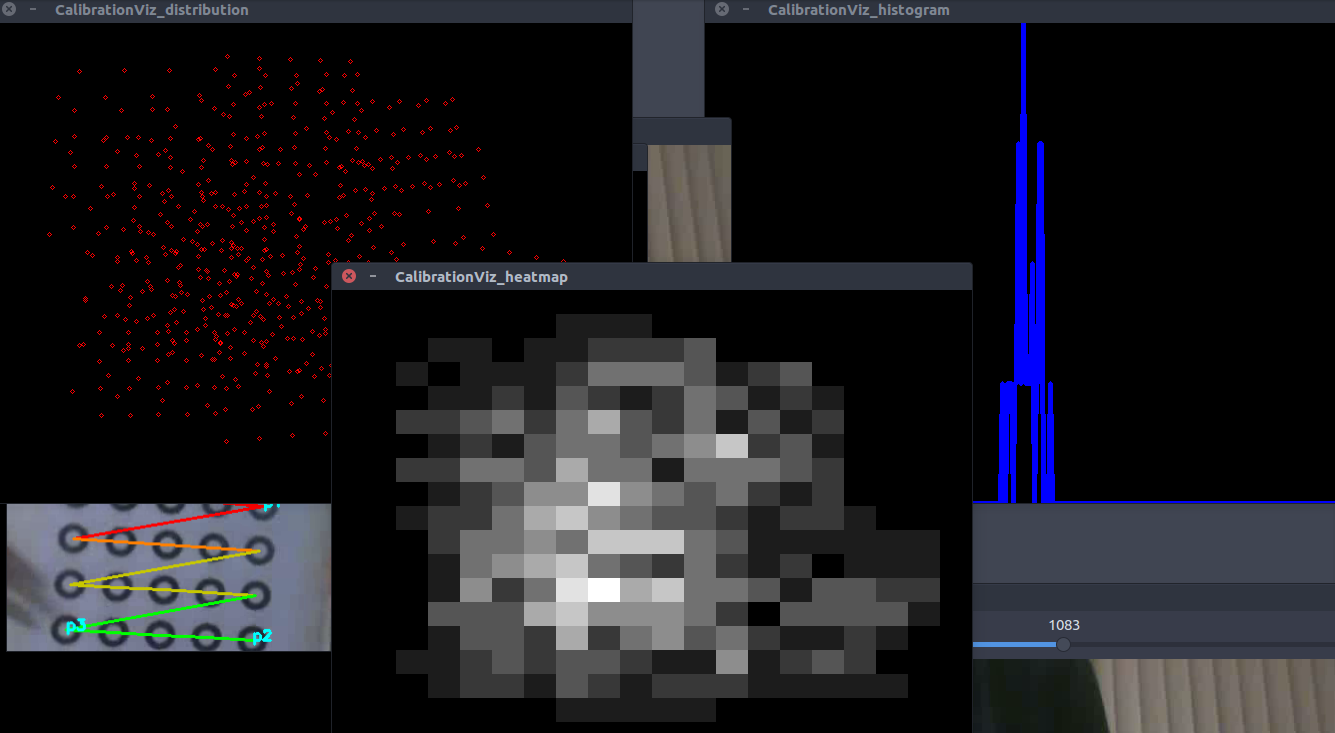
\includegraphics[width=2.5in]{_img/tools.png}
\caption{Pattern final ordering after matching.}
\end{figure}

We have a heat-map that give us a distribution visualizer, as well as a histogram to be sure we are picking the patterns at some range of orientations.

\IEEEtriggeratref{8}

% references section
\begin{thebibliography}{1}

\bibitem{OpenCV}
  Bradski, G. \\
  \textit{OpenCV library.} - 2000
\\
\bibitem{Prakash2012}
  Charan Prakash, Lina Karam\\
  \textit{Camera calibration using adaptive segmentation and ellipse fitting for localizing control points.} - 2012
\\
\bibitem{Ankur2009}
  Ankur Datta, Jun-Sik Kim, Takeo Kanade\\
  \textit{Accurate camera calibration using iterative refinement of control points.} - 2009
\\
\bibitem{CameraCalibration1}
  Zhengyou Zhang \\
  \textit{A Flexible New Technique for Camera Calibration.} - 2000
\\
\bibitem{IntegralImageThresholding}
  Derek Bradley, Gerhard Roth \\
  \textit{Adaptive Thresholding Using the Integral Image.} - 2011

\end{thebibliography}


\end{document}
